\documentclass[10pt,preprint]{aastex631}
\usepackage{amsmath,amsfonts,amssymb}
\usepackage{mathrsfs}
\DeclareMathAlphabet{\mathpzc}{OT1}{pzc}{m}{it}

\usepackage[]{graphicx, epstopdf}
\graphicspath{{Figures/}}

%\usepackage{indentfirst}
%\usepackage{lscape}
\usepackage{afterpage}
%\usepackage{rotating}
\let\captionbox\undefined
%\usepackage{caption}

\usepackage{datetime2}

%\captionsetup{width=6.3in,font=footnotesize}
%\usepackage{wrapfig}
%\usepackage{multicol}
%\usepackage{textcomp}
%\newcommand{\textapprox}{\raisebox{0.5ex}{\texttildelow}}

% custom commands for Jared's changes
%\usepackage{ulem}
%\newcommand{\jrmadd}[1]{\textcolor{blue}{#1}}
%\newcommand{\jrmrmv}[1]{\textcolor{blue}{\sout{#1}}}

% custom commands for Olivier's comments
%\usepackage{ulem}
%\newcommand{\ogadd}[1]{\textcolor{orange}{#1}}
%\newcommand{\ogrmv}[1]{\textcolor{orange}{\sout{#1}}}

% custom commends for Mike's comments
%\definecolor{avocado}{rgb}{0.34,0.51,0.01}
%\newcommand{\mpfadd}[1]{\textcolor{avocado}{#1}}
%\newcommand{\mpfrmv}[1]{\textcolor{avocado}{\sout{#1}}}

%\usepackage{multirow}

%\usepackage{xcolor}
%\usepackage{ulem}

%\usepackage{soul}

%\setlength{\textwidth}{6.5in}
%\setlength{\hoffset}{0in}
%\setlength{\oddsidemargin}{0in}
%\setlength{\evensidemargin}{0in}

%\setlength{\textheight}{9.in}
%\setlength{\voffset}{0in}
%\setlength{\topmargin}{0in}
%\setlength{\headsep}{0.25in}
%\setlength{\headheight}{0in}


%Some handy-dandy commands
%***Distance and Length***
\newcommand{\meters}{\mbox{m}}
\newcommand{\cm}{\mbox{cm}}
\newcommand{\km}{\mbox{km}}
\newcommand{\dpc}{d_{pc}}
\newcommand{\au}{\mbox{AU}}
\newcommand{\microns}{\mu\mbox{m}}
\newcommand{\rsun}{R_{\sun}}
\newcommand{\rjup}{R_J}
\newcommand{\rearth}{R_{\earth}}

%***Times***
\newcommand{\hours}{\mbox{ hrs}}
\newcommand{\seconds}{\mbox{ s}}
\newcommand{\years}{\mbox{ yrs}}

%**Mass**
\newcommand{\kg}{\mbox{kg}}
\newcommand{\msun}{M_{\sun}}
\newcommand{\mearth}{M_{\earth}}
\newcommand{\mjup}{M_J}



\newcommand{\lambdasci}{\lambda_\mathrm{sci}}
\newcommand{\lambdawfs}{\lambda_\mathrm{wfs}}
\newcommand{\tautd}{\tau_\mathrm{td}}
\newcommand{\tauwfs}{\tau_\mathrm{wfs}}
\newcommand{\dopt}{d_\mathrm{opt}}
\newcommand{\mmax}{m_\mathrm{max}}
\newcommand{\nmax}{n_\mathrm{max}}
\newcommand{\Ji}{\mathrm{Ji}}
\newcommand{\pone}{ {\scalebox{0.6}{+1}}}
\newcommand{\mone}{ {\scalebox{0.6}{-1}} }

\newcommand{\karman}{K\'{a}rm\'{a}n }


\newcommand{\argmax}{\operatornamewithlimits{argmax}}
\newcommand{\argmin}{\operatornamewithlimits{argmin}}



% Alter some LaTeX defaults for better treatment of figures:
    % See p.105 of "TeX Unbound" for suggested values.
    % See pp. 199-200 of Lamport's "LaTeX" book for details.
    %   General parameters, for ALL pages:
    \renewcommand{\topfraction}{0.9}    % max fraction of floats at top
    \renewcommand{\bottomfraction}{0.8} % max fraction of floats at bottom
    %   Parameters for TEXT pages (not float pages):
    \setcounter{topnumber}{2}
    \setcounter{bottomnumber}{2}
    \setcounter{totalnumber}{4}     % 2 may work better
    \setcounter{dbltopnumber}{2}    % for 2-column pages
    \renewcommand{\dbltopfraction}{0.9} % fit big float above 2-col. text
    \renewcommand{\textfraction}{0.07}  % allow minimal text w. figs
    %   Parameters for FLOAT pages (not text pages):
    \renewcommand{\floatpagefraction}{0.7}      % require fuller float pages
        % N.B.: floatpagefraction MUST be less than topfraction !!
    \renewcommand{\dblfloatpagefraction}{0.7}   % require fuller float pages





\begin{document}

\title{STP Coronagraph Pointing Control Envelope PSD Estimates \footnote{git state when this document was compiled: \input{../git_version.txt}}}

\author{Jared R. Males}

\begin{abstract}
Sweep analysis of input pointing PSD parameters to determine angle tracker and FSM control loop requirements.
Last updated \DTMnow.
\end{abstract}

\section{Control Model}

Some key assumptions are:
\begin{itemize}
\item A closed-loop feedback system with simple integrator control law, with gain optimized as in \citet{2018JATIS...4a9001M}.  See Figure \ref{fig:flowChart}.
\item FSM has negligible dynamics, and can be modeled as a sample-and-hold at relevant frequencies.
\end{itemize}

Important Caveats are:
\begin{itemize}
\item Resonances/peaks/poles/harmonic-vibrations will reduce temporal bandwidth, but higher order (predictive) filters can be used.  \\
\end{itemize}

\begin{figure}
\centering
\includegraphics[width=6.5in]{../flowChart/flowChart.pdf}
\vspace{-3cm}
\caption{Angle tracker based control flow.  Note that ``telescope disturbances'' are not explicitly modeled, but the input pointing PSDs should be assumed to model the combined effect of pointing and onboard jitter.  The FSM is modeled as a simple sample-and-hold, no other dynamics are included.  The loop delay was always set to twice the WFS exposure time.  \label{fig:flowChart}}
\end{figure}


\section{Input PSDs}

PSDs are modeled using the von Ka'rman model as in \citet{2019AJ....157...36D}, which as the form
\begin{equation}
\mathcal{T}(f) = \frac{\beta^2}{\left(f^2 + (1/T_0)^2\right)^{\alpha/2}}
\label{eqn:vkpsd}
\end{equation}
where $\beta$ is a normalization constant which controls the integrated variance, $T_0$ is a time constant that defines the knee frequency $1/T_0$, and $\alpha$ gives the PSD slope.

Larger $T_0$ can be thought of as a long-slow drift, whereas smaller $T_0$ will produce rapid stochastic fluctuations.  Larger $\alpha$ produce stronger correlations at frequencies higher than $1/T_0$, which provides for more control effectiveness.  Smaller $\alpha$ processes are harder to control.

\begin{figure}
\centering
\includegraphics[width=3.5in]{psdPrimer.pdf}
\caption{Example von Ka'rman PSDs demonstrating the effect of varying $T_0$ and $\alpha$.  All have the same integral (or total rms). Smaller $T_0$ (or higher knee frequencies) and smaller $\alpha$ (shallower slope) result in more power at higher frequencies.  This in turn makes control harder, requiring faster control loops. \label{fig:vkpsds}}
\end{figure}

An example spacecraft pointing PSD is shown in Figure \ref{fig:examp_psd}.

\begin{figure}
\centering
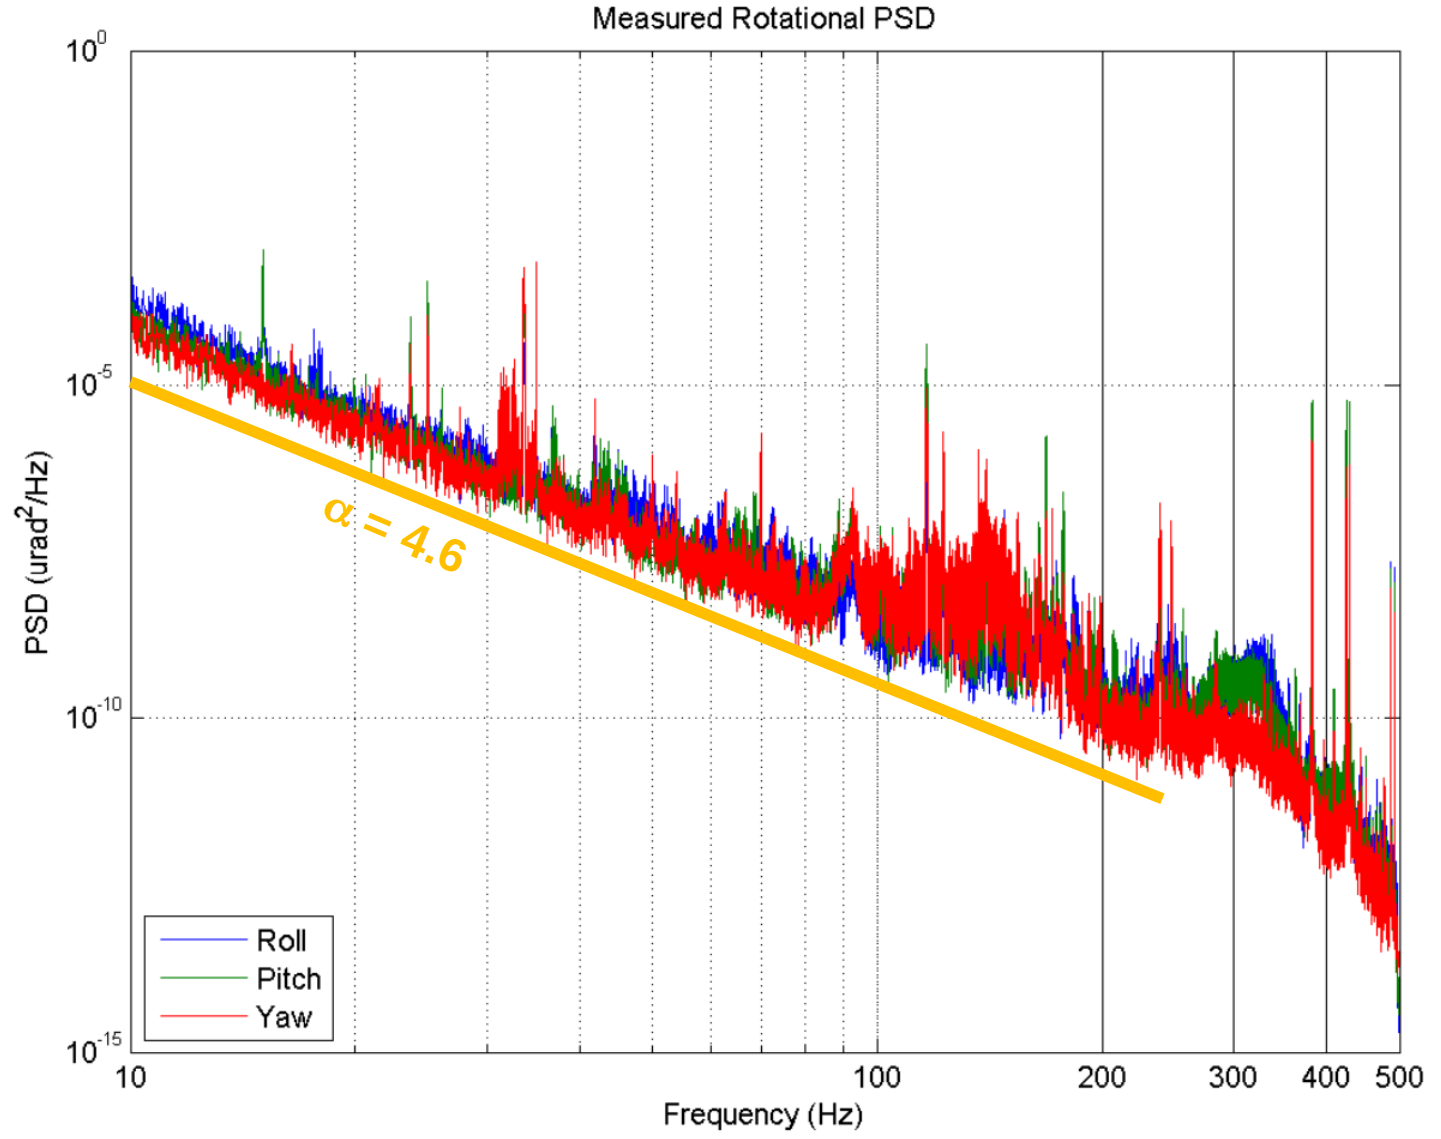
\includegraphics[width=3.5in]{ssl_example.png}
\caption{Example pointing PSD from SSL.  The gold line has a slope of approximately $\alpha=4.6$, and we can infer that $T_0 > 0.1$ sec.  Figure adapted from \citet{woo:2017}. \label{fig:examp_psd}}
\end{figure}

\section{Analysis}

A grid sweep analysis is conducted, where an input disturbance rms, a PSD slope $\alpha$, and a PSD knee frequency $T_0$ are chosen, and then a range of loop frequencies are tested.  At each loop frequency, gain is optimized, and then the lowest loop frequency needed to obtain the single-axis jitter at the coronagraph focal plane is recorded.

\clearpage

\section{Scenario 1: 10 nm rms OPD at 100 Hz on a 0 mag star}

\begin{table}[h!]
\begin{tabular}{lccl}
\hline
\hline
Parameter & Value & Units & Notes \\
\hline
M1 Diameter & 3.0 & m &\\
Filter      & r'  &   & using MagAO-X bandpass \\
$\lambda_0$  & 615.0 & nm & central wavelength \\
$\Delta \lambda$ &  111.0 & nm & effective filter width \\
Throughput  & 0.06 && throughput to the AT detector \\
Lyot Stop Refl. & 0.75 & & fraction of light reflected by Lyot Stop to AT detector \\
QE & 0.8 && QE of AT detector \\
$F_0$ & $2.2\times10^{9}$ & photons/sec & photon flux from a 0 Vega mag star at AT \\
star mag & 0 & Vega magnitudes & target star brightness in the filter \\
$\beta_p$ & 5 & & Sensor sensitivity. 5 is a fairly bad sensor. see \citep{2005ApJ...629..592G} \\
$n_{pix}$ & 1692 & pixels & number of pixels used for sensing \\
$\sigma_{ron}$ & 2 & electrons & readout noise of detector\\
$f_s$ & 100 & Hz & maximum loop speed \\
$\tau$ & $2/f_s$ & sec & loop delay between sensing and FSM update \\
$\sigma_{TT}$ & 10 & nm rms OPD & the required one-axis pointing residual\\
\hline
\end{tabular}
\end{table}

\begin{figure}[h!]
\centering
\includegraphics[width=6.5in]{../plots/3m_10nm_0mag_out_T0-100HzComp.pdf}
\caption{Contours showing which combination of PSD parameters which require a 100 Hz control loop frequency to achieve 10 nm OPD rms jitter using the coronagraph FSM (one-axis) as a function of input pointing error rms, PSD $\alpha$, and knee-frequency $1/T_0$. For a given $T_0$ value, PSDs below and to the right of curve will allow slower loop speeds.  This is shown in subsequent plots.  \label{fig:s1_T0-100HzComp}}
\end{figure}

\begin{figure}[h!]
\centering
\includegraphics[width=3in]{../plots/3m_10nm_0mag_out_T0_3000.000000.pdf}
\caption{Map of loop frequencies required to achieve 10 nm rms jitter using the coronagraph FSM (one-axis) as a function of input pointing error and PSD $\alpha$, for knee-frequency $T_0 = 3000$ sec.  Contours are drawn at 10,50,200,100, and 500 Hz (10 Hz is the lowest/right-most).  \label{fig:s1_T0-3000}}
\end{figure}

\begin{figure}[h!]
\centering
\includegraphics[width=3in]{../plots/3m_10nm_0mag_out_T0_1000.000000.pdf}
\caption{Map of loop frequencies required to achieve 10 nm rms jitter using the coronagraph FSM (one-axis) as a function of input pointing error and PSD $\alpha$, for knee-frequency $T_0 = 1000$ sec.  Contours are drawn at 10,50,200,100, and 500 Hz (10 Hz is the lowest/right-most).  \label{fig:s1_T0-1000}}
\end{figure}

\begin{figure}[h!]
\centering
\includegraphics[width=3in]{../plots/3m_10nm_0mag_out_T0_300.000000.pdf}
\caption{Map of loop frequencies required to achieve 10 nm rms jitter using the coronagraph FSM (one-axis) as a function of input pointing error and PSD $\alpha$, for knee-frequency $T_0 = 300$ sec.  Contours are drawn at 10,50,200,100, and 500 Hz (10 Hz is the lowest/right-most).  \label{fig:s1_T0-300}}
\end{figure}

\begin{figure}[h!]
\centering
\includegraphics[width=3in]{../plots/3m_10nm_0mag_out_T0_100.000000.pdf}
\caption{Map of loop frequencies required to achieve 10 nm rms jitter using the coronagraph FSM (one-axis) as a function of input pointing error and PSD $\alpha$, for knee-frequency $T_0 = 100$ sec.  Contours are drawn at 10,50,200,100, and 500 Hz (10 Hz is the lowest/right-most).  \label{fig:s1_T0-100}}
\end{figure}

\begin{figure}[h!]
\centering
\includegraphics[width=3in]{../plots/3m_10nm_0mag_out_T0_30.000000.pdf}
\caption{Map of loop frequencies required to achieve 10 nm rms jitter using the coronagraph FSM (one-axis) as a function of input pointing error and PSD $\alpha$, for knee-frequency $T_0 = 30$ sec.  Contours are drawn at 10,50,200,100, and 500 Hz (10 Hz is the lowest/right-most).  \label{fig:s1_T0-30}}
\end{figure}

\begin{figure}[h!]
\centering
\includegraphics[width=3in]{../plots/3m_10nm_0mag_out_T0_10.000000.pdf}
\caption{Map of loop frequencies required to achieve 10 nm rms jitter using the coronagraph FSM (one-axis) as a function of input pointing error and PSD $\alpha$, for knee-frequency $T_0 = 10$ sec.  Contours are drawn at 10,50,200,100, and 500 Hz (10 Hz is the lowest/right-most).  \label{fig:s1_T0-10}}
\end{figure}

\begin{figure}[h!]
\centering
\includegraphics[width=3in]{../plots/3m_10nm_0mag_out_T0_3.000000.pdf}
\caption{Map of loop frequencies required to achieve 10 nm rms jitter using the coronagraph FSM (one-axis) as a function of input pointing error and PSD $\alpha$, for knee-frequency $T_0 = 3$ sec.  Contours are drawn at 10,50,200,100, and 500 Hz (10 Hz is the lowest/right-most).  \label{fig:s1_T0-1}}
\end{figure}

\begin{figure}[h!]
\centering
\includegraphics[width=3in]{../plots/3m_10nm_0mag_out_T0_1.000000.pdf}
\caption{Map of loop frequencies required to achieve 10 nm rms jitter using the coronagraph FSM (one-axis) as a function of input pointing error and PSD $\alpha$, for knee-frequency $T_0 = 1$ sec.  Contours are drawn at 10,50,200,100, and 500 Hz (10 Hz is the lowest/right-most).  \label{fig:s1_T0-1}}
\end{figure}

\clearpage
\section{Scenario 1: 10 nm rms OPD at 100 Hz on a 5th mag star}

There is only a negligible difference in results on a 5th mag star.

\begin{table}[h!]
\begin{tabular}{lccl}
\hline
\hline
Parameter & Value & Units & Notes \\
\hline
M1 Diameter & 3.0 & m &\\
Filter      & r'  &   & using MagAO-X bandpass \\
$\lambda_0$  & 615.0 & nm & central wavelength \\
$\Delta \lambda$ &  111.0 & nm & effective filter width \\
Throughput  & 0.06 && throughput to the AT detector \\
Lyot Stop Refl. & 0.75 & & fraction of light reflected by Lyot Stop to AT detector \\
QE & 0.8 && QE of AT detector \\
$F_0$ & $2.2\times10^{9}$ & photons/sec & photon flux from a 0 Vega mag star at AT \\
star mag & 5 & Vega magnitudes & target star brightness in the filter \\
$\beta_p$ & 5 & & Sensor sensitivity. 5 is a fairly bad sensor. see \citep{2005ApJ...629..592G}. \\
$n_{pix}$ & 1692 & pixels & number of pixels used for sensing \\
$\sigma_{ron}$ & 2 & electrons & readout noise of detector\\
$f_s$ & 100 & Hz & maximum loop speed \\
$\tau$ & $2/f_s$ & sec & loop delay between sensing and FSM update \\
$\sigma_{TT}$ & 10 & nm rms OPD & the required one-axis pointing residual\\
\hline
\end{tabular}
\end{table}

\begin{figure}[h!]
\centering
\includegraphics[width=6.5in]{../plots/3m_10nm_5mag_out_T0-100HzComp.pdf}
\caption{Contours showing which combination of PSD parameters which require a 100 Hz control loop frequency to achieve 10 nm OPD rms jitter using the coronagraph FSM (one-axis) as a function of input pointing error rms, PSD $\alpha$, and knee-frequency $1/T_0$. For a given $T_0$ value, PSDs below and to the right of curve will allow slower loop speeds.  This is shown in subsequent plots.  \label{fig:s2_T0-100HzComp}}
\end{figure}

\begin{figure}[h!]
\centering
\includegraphics[width=3in]{../plots/3m_10nm_5mag_out_T0_3000.000000.pdf}
\caption{Map of loop frequencies required to achieve 10 nm rms jitter using the coronagraph FSM (one-axis) as a function of input pointing error and PSD $\alpha$, for knee-frequency $T_0 = 3000$ sec.  Contours are drawn at 10,50,200,100, and 500 Hz (10 Hz is the lowest/right-most).  \label{fig:s2_T0-3000}}
\end{figure}

\begin{figure}[h!]
\centering
\includegraphics[width=3in]{../plots/3m_10nm_5mag_out_T0_1000.000000.pdf}
\caption{Map of loop frequencies required to achieve 10 nm rms jitter using the coronagraph FSM (one-axis) as a function of input pointing error and PSD $\alpha$, for knee-frequency $T_0 = 1000$ sec.  Contours are drawn at 10,50,200,100, and 500 Hz (10 Hz is the lowest/right-most).  \label{fig:s2_T0-1000}}
\end{figure}

\begin{figure}[h!]
\centering
\includegraphics[width=3in]{../plots/3m_10nm_5mag_out_T0_300.000000.pdf}
\caption{Map of loop frequencies required to achieve 10 nm rms jitter using the coronagraph FSM (one-axis) as a function of input pointing error and PSD $\alpha$, for knee-frequency $T_0 = 300$ sec.  Contours are drawn at 10,50,200,100, and 500 Hz (10 Hz is the lowest/right-most).  \label{fig:s2_T0-300}}
\end{figure}

\begin{figure}[h!]
\centering
\includegraphics[width=3in]{../plots/3m_10nm_5mag_out_T0_100.000000.pdf}
\caption{Map of loop frequencies required to achieve 10 nm rms jitter using the coronagraph FSM (one-axis) as a function of input pointing error and PSD $\alpha$, for knee-frequency $T_0 = 100$ sec.  Contours are drawn at 10,50,200,100, and 500 Hz (10 Hz is the lowest/right-most).  \label{fig:s2_T0-100}}
\end{figure}

\begin{figure}[h!]
\centering
\includegraphics[width=3in]{../plots/3m_10nm_5mag_out_T0_30.000000.pdf}
\caption{Map of loop frequencies required to achieve 10 nm rms jitter using the coronagraph FSM (one-axis) as a function of input pointing error and PSD $\alpha$, for knee-frequency $T_0 = 30$ sec.  Contours are drawn at 10,50,200,100, and 500 Hz (10 Hz is the lowest/right-most).  \label{fig:s2_T0-30}}
\end{figure}

\begin{figure}[h!]
\centering
\includegraphics[width=3in]{../plots/3m_10nm_5mag_out_T0_10.000000.pdf}
\caption{Map of loop frequencies required to achieve 10 nm rms jitter using the coronagraph FSM (one-axis) as a function of input pointing error and PSD $\alpha$, for knee-frequency $T_0 = 10$ sec.  Contours are drawn at 10,50,200,100, and 500 Hz (10 Hz is the lowest/right-most).  \label{fig:s2_T0-10}}
\end{figure}

\begin{figure}[h!]
\centering
\includegraphics[width=3in]{../plots/3m_10nm_5mag_out_T0_3.000000.pdf}
\caption{Map of loop frequencies required to achieve 10 nm rms jitter using the coronagraph FSM (one-axis) as a function of input pointing error and PSD $\alpha$, for knee-frequency $T_0 = 3$ sec.  Contours are drawn at 10,50,200,100, and 500 Hz (10 Hz is the lowest/right-most).  \label{fig:s2_T0-1}}
\end{figure}

\begin{figure}[h!]
\centering
\includegraphics[width=3in]{../plots/3m_10nm_5mag_out_T0_1.000000.pdf}
\caption{Map of loop frequencies required to achieve 10 nm rms jitter using the coronagraph FSM (one-axis) as a function of input pointing error and PSD $\alpha$, for knee-frequency $T_0 = 1$ sec.  Contours are drawn at 10,50,200,100, and 500 Hz (10 Hz is the lowest/right-most).  \label{fig:s2_T0-1}}
\end{figure}
\clearpage

\bibliographystyle{apj}
\bibliography{pointingEnv}



\end{document}
